\documentclass[11pt]{article}
\usepackage{graphicx} % This lets you include figures
\usepackage{hyperref} % This lets you make links to web locations
\usepackage[margin=0.5in]{geometry}
\usepackage[rightcaption]{sidecap}
\usepackage{subcaption}
\usepackage{wrapfig}
\usepackage{float}
\usepackage{imakeidx}
\usepackage{indentfirst}
\makeindex
%---------------------------Do Not Edit Anything Above This Line!!------------------------

% edit the line below, if needed, to change the directory name for your image files.
\graphicspath{ {./images/} }



\begin{document}

%---------------------------Edit Content in the Box to Create the Title Page--------------
\begin{titlepage}
   \begin{center}
       \vspace*{1cm}
	   \Huge
       \textbf{GPS Based Campus Room Finder}

       \vspace{0.5cm}
       \Large
       Sprint  1 \\
       2025-09-02 \\
   \end{center}

       \vspace{1.5cm}

\begin{table}[h!]
\centering
\begin{tabular}{|l|l|}
\hline
\textbf{Name} & \textbf{Email Address} \\ \hline
Aaron Downing         & aaron.downing652@topper.wku.edu         \\ \hline
Ryerson Brower         & ryerson.brower178@topper.wku.edu         \\ \hline
Kaden Hunt         & kaden.hunt144@topper.wku.edu         \\ \hline
\end{tabular}
\end{table}

%Latex Table Generator    
%https://www.tablesgenerator.com/     
        
\vspace{4in}

\centering  
Michael Galloway \\
CS 361 \\
Fall 2025\\
Project Technical Documentation

\end{titlepage}
%---------------------------Edit Content in the Box to Create the Title Page--------------


% No text here.


%---------------------------Do Not Edit Anything In This Box!!------------------------
%Table of contents and list of figures will be autogenerated by this section.
\newpage
\setcounter{page}{1}%
\cleardoublepage
\pagenumbering{gobble}
\tableofcontents
\cleardoublepage
\pagenumbering{arabic}
\clearpage
\newpage
\setcounter{page}{1}%
\cleardoublepage
\pagenumbering{gobble}
\listoffigures
\cleardoublepage
\pagenumbering{arabic}
\newpage
%---------------------------Do Not Edit Anything In This Box!!------------------------




%---------------------------Project Introduction Section------------------------------

% No text here.

\section{Introduction} %\section{} is used to create major section headers

% No text here.

%---------------------------Project Overview------------------------------------------
\subsection{Project Overview} %\subsection{} is used to create minor sections 
% 300 words
% Description of the project, what the project provides, its purpose, problems solved, and target audience.

The GPS Based Campus Room Finder is a mobile application designed to simplify navigation for WKU students and faculty. The primary purpose of this project is to create a consistent and easy-to-use tool that addresses the common problem of navigating a large and unfamiliar campus environment. Using GPS technology, the application will help users quickly determine their current location and find the most efficient route to any building and room number on campus. This tool will eliminate the need for paper maps and provide an important resource for new and current members of WKU.
%use blank lines to begin a new paragraph

The final product will be a user-friendly mobile application that gives real-time guidance and an estimation of travel times. This software will be a valuable tool for the university with potential for expansion to include additional features that continue to enhance the campus experience.
%---------------------------End Project Overview---------------------------------------

% No text here.

%---------------------------Project Scope----------------------------------------------
\subsection{Project Scope}
% 350 words
% Description of all deliverables, benefits, outcomes, and work required (all tasks, costs, time, people, resources, dates/deadlines, and final deliverables date).

The project scope defines the boundaries, commitments, and outputs required to deliver the GPS-Based Campus Room Finder. This scope covers all activities necessary to design, implement, test, and document a mobile application that meets the client's expectations while remaining usable and maintainable beyond the project timeline.

\textbf{Deliverables \& Outcomes:}
\begin{itemize}
    \item \textbf{Written Reports:} Detailed organizational and technical documents submitted at the conclusion of each of the four sprints.
    \item \textbf{Presentations:} A presentation delivered at the end of each sprint to summarize progress and demonstrate results.
    \item \textbf{Evaluations:} Peer evaluation forms submitted individually by team members after each sprint.
    \item \textbf{Final Product:} A fully tested, documented, and maintainable Android mobile application that provides GPS-based navigation to campus buildings and rooms.
\end{itemize}

\textbf{Work Required:}
\begin{itemize}
    \item \textbf{Tasks:} All development tasks including source code creation, user interface design, system integration, testing, and documentation. Additional requirements will be integrated as identified throughout the project.
    \item \textbf{Team:} 
        \begin{itemize}
            \item Kaden Hunt — Project Manager, Task Manager
            \item Aaron Downing — Documentation Draft
            \item Ryerson Brower — Research Coordinator
        \end{itemize}
    \item \textbf{Time Commitment:} Work will be divided across four sprints. Each team member will contribute 8–10 hours per week to development, meetings, and documentation.
    \item \textbf{Resources:} GitHub will serve as the version control system and task management platform. The documentation will be written collaboratively in Texmaker. The development will take place on personal laptops running Windows 10 or later which will meet the requirements of Android Studio. of Android Studio.
    \item \textbf{Schedule:} Deliverables align with the four milestone deadlines outlined on Blackboard. Weekly client meetings occur on Tuesdays at 12:35 p.m. in Snell Hall B104. Internal team meetings will take place on Thursdays at 2:00 p.m.
\end{itemize}

Altogether, this scope establishes what will be delivered, the benefits it provides, and the foundation for successful implementation
%---------------------------End Project Scope---------------------------------------

% No text here.


\subsection{Technical Requirements}


%---------------------------Functional Requirements----------------------------------------------
\subsubsection{Functional Requirements} %\subsubsection{} used to create sections for parent subsections.
% Functional requirements define what a system or software must do, specifying the desired behavior or functionality.

% List as atomic bullet points that can be tested

\begin{table}[h!]
\centering
\begin{tabular}{|l|}
\hline
\textbf{Mandatory Functional Requirements} \\ \hline
The application will use GPS coordinates to determine the user’s current location within the campus boundaries.                                     \\  \hline
The application will allow the user to search for a specific building and room number using a text-based input.                                      \\ \hline
The application will generate a step-by-step navigation route from the user’s current location to the selected room.                                     \\ \hline
The application will have an interactive display to navigate the user to the building and room.                                           \\ \hline
The application will provide an estimated travel time based on the mobile location of the user.                                           \\ \hline
\textbf{Extended Functional Requirements}  \\ \hline
The application will provide voice-guided navigation for hands-free use.                                 \\ \hline
The application will allow users to bookmark or “favorite” frequently visited rooms for quicker searches.                                 \\ \hline
The application will provide a “recent searches” history so users can quickly reselect prior destinations                                 \\ \hline
                                           
\end{tabular}
\end{table}

% Paragraph (150 words) explaining the need and purpose for the listed Functional Requirements.
The functional requirements for the WKU GPS-based campus room finder are designed to help WKU students and faculty easily locate rooms across campus. By using GPS coordinates to determine the user's current location, the application provides accurate, real-time directions, allowing users to navigate campus quickly and effectively. The interactive display offers clear step-by-step guidance to the desired building and room number, featuring a user-friendly interface that makes input, ensuring easy accessibility for all users. To get rid of any other unnecessary confusion, the application will provide an estimated travel time based on the mobile location of the user. This feature also allows users to make better decisions about which route to take depending on their time constraints between classes. The applications goal is to address common problems such as getting lost or arriving late to class, enhancing convenience and creating a smoother, more reliable navigation experience across the WKU campus.


%---------------------------End Functional Requirements----------------------------------------------

% No text here.

%---------------------------Non-Functional Requirements----------------------------------------------
\subsubsection{Non-Functional Requirements}
% Non-functional requirements specify the constraints, qualities, or attributes that the system or software must possess, such as performance, security, usability, portability, fault tolerance, or reliability.

% List as atomic bullet points that can be tested

\begin{table}[h!]
\centering
\begin{tabular}{|l|}
\hline
\textbf{Mandatory Non-Functional Requirements} \\ \hline
The application will provide location updates with an accuracy of at least ±5 meters under clear sky conditions.                                      \\ \hline
The application will deliver route generation results within 2 seconds of the user’s search request.                                      \\ \hline
The application will be compatible with either Android or iOS mobile operating systems.                                      \\ \hline
The application will provide visual and text-based route guidance.                                           \\ \hline
The application will support operation in both portrait and landscape orientations without loss of functionality.                                           \\ \hline
All project source code must be developed by the CS 360 project team.                                           \\ \hline
The project must use a database.                                           \\ \hline
Performance metrics should be gathered and optimized.                                          \\ \hline
Security metrics should be gathered and optimized                                           \\ \hline
User interface metrics should be gathered and optimized.                                           \\ \hline
\textbf{Extended Non-Functional Requirements}  \\ \hline
The application should maintain functionality with limited or no internet connection                                 \\ \hline
The application should consume minimal battery power while running in the background.                                 \\ \hline
The application should be designed with a clean, intuitive user interface that prioritizes ease of use.                                 \\ \hline

\end{tabular}
\end{table}

% Paragraph (150 words) explaining the need and purpose for the listed Non-Functional Requirements.
The mandatory non functional requirements for the WKU GPS-based campus room finder ensure the application performs reliably, efficiently, and securely while providing users with a positive application experience. By requiring location updates with an accuracy of within 5 meters under clear sky conditions, the app guarantees precise position for navigating campus. Delivering route generation results within 2 seconds ensures that users receive routes efficiently without unnecessary delays. Visual and text-based route guidance enhances accessibility and makes navigation possible for all users. Requiring all project source  code must be developed by the CS 360 project team helps achieve the desired learning outcomes of the class and encourages accountability throughout the team in a real-world setting. Using a database enables efficient storage and retrieval of all building and rooms on campus. Additionally, gathered and optimized security metrics will ensure the application remains fast, safe, and easy to use, while also meeting quality standards set out by the client. Collectively, these requirements provide a reliable and high-quality tool for campus navigation.
%use blank lines to begin a new paragraph


%---------------------------End Non-Functional Requirements---------------------------------------

% No text here.

%---------------------------Target Hardware Details----------------------------------------------
\subsection{Target Hardware Details}
% 200 words
% CPU (if a specific architecture is needed), RAM (required while the product is running), Persistent Storage Space, Network connection (Wi-Fi, Ethernet), Network bandwidth (required while the product is running), Output devices (Monitor (how many? What resolution?), speakers, VR headset), Input devices (Keyboard, mouse, touchscreen, VR headset).  Create test cases for each to verify.
We will create a mobile app for students and faculty around campus. The target hardware for our mobile app will primarily be for smart phones on Android. The inimume requrimenst are:

- The minimum CPU required is a quad-core ARM-based processor (or the processor that's in most smart phones) to ensure real time GPS processing and navigation. Our test case for the CPU would be to run a continuous navigation to confirm smooth updating with no lag. 

- You would need at least 2 GB of RAM so the product can also run things like GPS tracking at the same time and the rendering of the map. Our test case for the RAM would be to monitor memory usage under a heavy load. 

- A minimum of 200 MB of persistent storage is needed for the application installation, location files, and maps. Our storage test case would be to install the app and see how much it takes up. 

- Network connectivity will be necessary via Wi-Fi or 4G/5G mobile data, with at least 1 Mbps of sustained bandwidth for map updates and routing queries. 
The targeted output device will be a touchscreen of a smart phone. 

We don't have a plan to place this app on PC or computers but it would be something to possible implement in the future. A software we are using called 

Android studios also has some hardware requirement. These are:

- A OS of 64-bit Windows 10 or newer. 

- RAM with 16 GB
 
- a CPU with a processor with visualization support (Intel VT-x or AMD-V)

- micro architecture from after 2017. 

- 16 GB of free disk space, preferably on a Solid State Drive (SSD). 

- A GPU with at least 4 GB of VRAM.
 

%---------------------------End Target Hardware Details----------------------------------------------

% No text here.

%---------------------------Software Product Deveopment----------------------------------------------
\subsection{Software Product Development}
% 200 words
% List the following used with their purpose for development: IDEs, IDE plugins, Software Languages, Software Frameworks, Version Control, Asset Generation Tools, and tools for colaboration (Google Drive, One Drive, GitHub, etc.).  Describle how each tool is used within your team.
The software we are using already are Google doc, TexLive, github, Android Studio, SQL and VScode. 

- Google doc we use to keep up with each others documents and any document we need to print out. 

- For our documentations we are using TexLive to edit both or Organizational and Tech Docs. 

- Github we used to get a repository that is easy to access and easy for us to place our updated docs and code. Git hub also helps use be able to access everything without having to send files back and forth.  

- We already planed on using VScode and the coding language we will use to code our app is JAVA. VS code with the help of github makes it really easy to pull everyone's code when they edit it so once again we are not sending a ton of files and getting them mixed up. 

- One of the more important software we will use is Android Studio. This will allow use to code and Android app easier. This will also let use visualize the app when we don't have a Android phone accessible. 

- For our database to hold all the data for location of rooms and routes we will use SQL.  

%---------------------------End Software Product Deveopment-----------------------------------------

% No text here.

%---------------------------End Project Introduction Section----------------------------------------


% No text here.





%---------------------------Modeling and Design Section------------------------------
\section{Modeling and Design}
% No text here.


%---------------------------System Boundaries------------------------------
\subsection{System Boundaries}

\subsubsection{Physical}
%100 words
% Describe the Physical System Boundaries.
The physical system boundaries for the GPS-Based Campus Room finder are limited to mobile devices, primarily Android smart phones used by WKU students and faculty. The application relies on the mobile phones built-in hardware components such as the GPS system, touchscreen interface, and mobile network for accurate navigation. It will not include any external hardware devices not included in the user's smart phone. The system interacts with Google Maps API (or similar) for real-time navigation and requires the campus buildings and room data stored in the project database. Any devices outside of android mobile devices, such as iphones, PCs, and kiosks, lie out of the scope of the project. The application requires minimum resources, 2GB of RAM and 100mb of storage will be enough which is available on most android phones. Security is ensured by relying on the built-in authentication systems on the phone. The application is easily scalable by adding functionality for more android phones and adding a larger database. 

%uncomment the section below when you're ready to insert an image
%\begin{figure}[h!]
%    \centering
%    \includegraphics[width=1\textwidth]{images/picture_of_Physical_boundaries.png}
%    \caption{Description of the image here.}
%    \label{phy_boundaries}
%\end{figure}






\subsubsection{Logical}
%100 words
% Describe the Logical System Boundaries.
The logical system boundaries for the GPS-Based Campus Room Finder defines the flow of the information and functions managed by the application. Internally, the system handles location detection, room and building searches, and route generation. It manages the retrieval of the campus building and room number data from the project database and uses the GPS coordinates for navigation. Externally, the system communicates with Google Maps API and user-interface to display directions and built-in mobile operating systems for device-level functions such as notifications. Any process beyond navigation, such as class scheduling and campus event times remain outside the logical scope of the project.

%uncomment the section below when you're ready to insert an image
%\begin{figure}[h!]
%    \centering
%    \includegraphics[width=1\textwidth]{images/picture_of_Logical_boundaries.png}
%    \caption{Description of the image here.}
%    \label{log_boundaries}
%\end{figure}

%---------------------------End System Boundaries------------------------------

% No text here.

%---------------------------Wireframes and Storyboard----------------------------------
\subsection{Wireframes and Storyboard}
%150 words
% Use wireframes to create scenes and images of the user interface.  Connect the wireframes to show progression through the product to create a storyboard.  Describe the wireframes and storyboard.
Text goes here.

%uncomment the section below when you're ready to insert an image
%\begin{figure}[h!]
%    \centering
%    \includegraphics[width=1\textwidth]{images/picture_of_storyboard.png}
%    \caption{Description of the image here.}
%    \label{storyboard}
%\end{figure}

%---------------------------End Wireframes and Storyboard----------------------------------

% No text here.

%---------------------------Unified Modeling Language----------------------------------
\subsection{UML}

\subsubsection{Class Diagrams}
%At least one for each design pattern category.   
%Each class diagram should include the following:
%	Title for each Class Diagram
%	Description of how and why each class is used
%	Mapping to source code (in the Appendix, specific files and line numbers) of where it’s used.
Text goes here.

%uncomment the section below when you're ready to insert an image
%\begin{figure}[h!]
%    \centering
%    \includegraphics[width=1\textwidth]{images/class_diagram.png}
%    \caption{Description of the image here.}
%    \label{class_diagram}
%\end{figure}


\subsubsection{Use Case Diagrams}
%Enough to cover all technical functional requirements.
%Each Use Case Diagram should include the following:
%	Title for each Use Case Diagram
%	A description of information given in the diagram.
%	Mapping to source code (in the Appendix, specific files and line numbers) of where it’s used.
Text goes here.

%uncomment the section below when you're ready to insert an image
%\begin{figure}[h!]
%    \centering
%    \includegraphics[width=1\textwidth]{images/use_case_diagram.png}
%    \caption{Description of the image here.}
%    \label{use_case_diagram}
%\end{figure}


\subsubsection{Use Case Scenarios Developed from Use Case Diagrams (Primary, Secondary)}
%Should include at least one primary and zero to many secondary scenarios
%Each Use Case Scenario should include the following:
%	Title for each Use Case Scenario
%	A short description of the information given in the scenario.
%	Mapping to source code (in the Appendix, specific files and line numbers) of where it’s used
Text goes here.

%uncomment the section below when you're ready to insert an image
%\begin{figure}[h!]
%    \centering
%    \includegraphics[width=1\textwidth]{images/use_case_scenario.png}
%    \caption{Description of the image here.}
%    \label{use_case_scenario}
%\end{figure}


\subsubsection{Sequence Diagrams}
%Each diagram should include all actors/resources to cover one Use Case Scenario.
%	Each Sequence Diagram should include the following:
%	Title for each Sequence Diagram
%	A short description of the information given in the diagram.
%	Mapping to source code (in the Appendix, specific files and line numbers) of where it’s used
Text goes here.

%uncomment the section below when you're ready to insert an image
%\begin{figure}[h!]
%    \centering
%    \includegraphics[width=1\textwidth]{images/use_case_scenario.png}
%    \caption{Description of the image here.}
%    \label{use_case_scenario}
%\end{figure}

\subsubsection{State Diagrams}
%Each diagram should identify the object/resource/asset (in the title of the diagram) and display all states and actions/events that create state changes.
%	Each State Diagram should include the following:
%	Title for each State Diagram
%	A short description of the information given in the diagram
%	Mapping to source code (in the Appendix, specific files and line numbers) of where it’s used
The following state diagram models the process of a user searching for a campus room. 
The diagram begins when the user enters a room number and submits it. 
The system then validates the input: if it is invalid, the user is prompted to retry; if valid, the system queries the database. 
If the room is found, a path is generated and directions are displayed. 
If the room is not found, or a query fails, the user can correct their input and resubmit. 
This diagram focuses only on the search and route-display feature in Sprint 2, since implementation has not yet begun. 

\begin{figure}[h!]
    \centering
    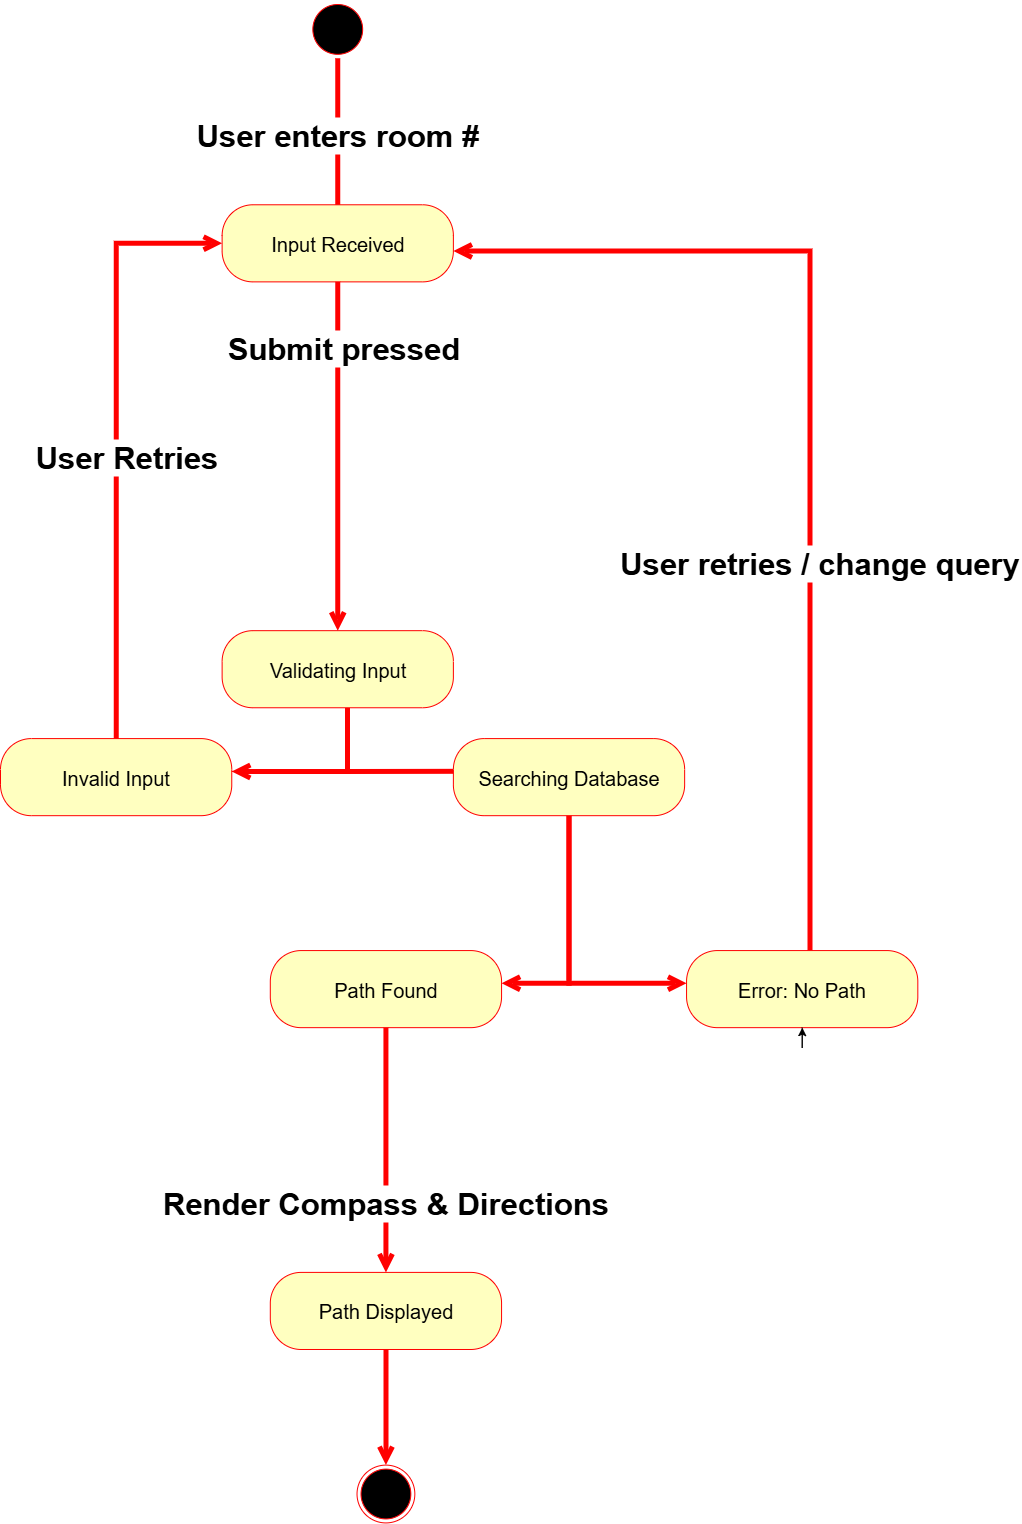
\includegraphics[width=0.4\textwidth]{images/state_diagram.png}
    \caption{State diagram for the room search feature, showing user input, validation, query, error handling, and path display.}
    \label{state_diagram}
\end{figure}

\subsubsection{Component Diagrams}
%Single diagram that defines component APIs and communication pathways for all software and dependencies used in the product.
%	The Component Diagram should include the following:
%	Title for the Component Diagram
%	A description of the information given in the diagram
%	Protocols used for each communication pathway
%	Mapping to all source code and dependency software (in the Appendix, specific files)
Text goes here.

%uncomment the section below when you're ready to insert an image
%\begin{figure}[h!]
%    \centering
%    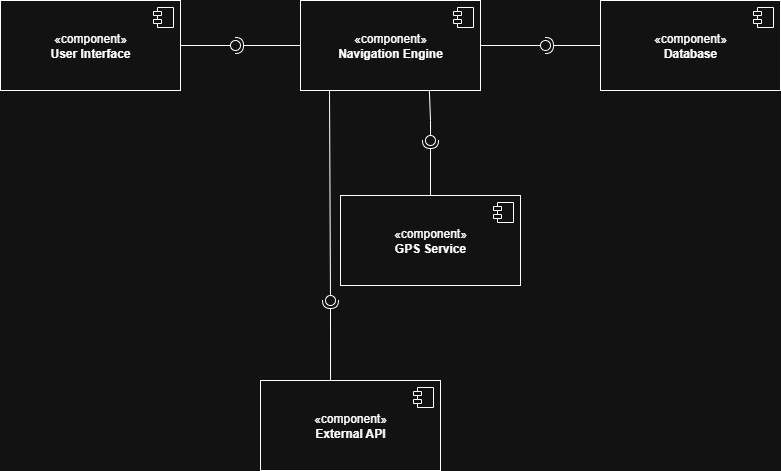
\includegraphics[width=1\textwidth]{images/component_diagram.png}
%    \caption{Description of the image here.}
%    \label{component_diagram}
%\end{figure}

\subsubsection{Deployment Diagrams}
%Single diagram that defines the physical nodes, virtual nodes, and communication for all software related to the product.  Should be an extension of the Component Diagram.
%	The Deployment Diagram should include the following:
%	Title for the Deployment Diagram
%	A description of the information given in the diagram
%	Identify all physical and virtual nodes used for process execution
%	Identify all internal and external node communication
Text goes here.

%uncomment the section below when you're ready to insert an image
%\begin{figure}[h!]
%    \centering
%    \includegraphics[width=1\textwidth]{images/deployment_diagram.png}
%    \caption{Description of the image here.}
%    \label{deployment_diagram}
%\end{figure}


%---------------------------End Unified Modeling Language----------------------------------

% No text here.

%---------------------------Version Control------------------------------------------------
\subsection{Version Control}
%150 words
%Describe your group's approach to version control.  Include details on how and when you make commits to GitHub.  Explain version naming, branching, and integration approaches.
Text goes here.


%---------------------------End Version Control------------------------------------------------

% No text here.

%---------------------------Requirments Traceability------------------------------------------------
\subsection{Requirements Traceability Table}
%150 words and table
%	Create a table that compares all requirements to use cases to make sure there are no missing features.
Text and table goes here.


%---------------------------End Data Dictionary------------------------------------------------


% No text here.

%---------------------------Data Dictionary------------------------------------------------
\subsection{Data Dictionary}
%150 words and table
%	Create a table that displays your Data Dictionary and describe how it is being used to define data structures and other major variables/elements in the software product.
Text and table goes here.


%---------------------------End Data Dictionary------------------------------------------------


% No text here.


%---------------------------User Experience Details------------------------------------------------
\subsection{User Experience}

\subsubsection{Gameplay Diagram}
%100 words
%Also called a controlled flow graph.  Insert an image of the gameplay diagram and describe the diagram in detail.
Text goes here.

%uncomment the section below when you're ready to insert an image
%\begin{figure}[h!]
%    \centering
%    \includegraphics[width=1\textwidth]{images/gameplay_diagram.png}
%    \caption{Description of the image here.}
%    \label{gameplay_diagram}
%\end{figure}

\subsubsection{Gameplay Objectives}
%100 words
%Should explain why someone should play your game. Should define the goals of your game.
Text goes here.

\subsubsection{User Skillset}
%100 words
%Describe the abilities a user should have in order to interact with the software: Screen tapping, Memorization, Puzzle, solving, Strategy development, Quick reflexes 
Text goes here.

\subsubsection{Gameplay mechanics}
%100 words
%Thorough guide of the game rules: Turn-based, Random chances, Capturing/eliminating, Time-based, Team-based
Text goes here.

\subsubsection{Gameplay Items}
%100 words
%This section of the GDD refers to smaller elements of the game, such as: Health/power-ups, Coins, Loot crates, Weapons/character upgrades, Etc. Changes gameplay elements as the player progresses through the game.
Text goes here.

\subsubsection{Gameplay Challenges}
%100 words
%Description of game challenges as a player progresses. Identify how a player handles difficulties and ensures the player can obtain essential tools to continue progressing through the game.
Text goes here.

\subsubsection{Gameplay Menu Screens}
%100 words and wireframes
%Game start menu screen, pause menu screen, game over screen
%Give wireframe/drawing/image for all menus in the game.
Text goes here.

\subsubsection{Gameplay Heads-Up Display}
%100 words and wireframes
%Current Game information visually relayed to the player as a part of the game’s user interface.
%HUD features are generally static, on-screen so they remain visible during gameplay. Health/Lives, Time, Weapons/Ammo, Capabilities, Menus, Mini-Map, Score, etc.
Text goes here.

\subsubsection{Gameplay Art Style}
%50 words
%describe the visual appearance of characters, objects, and other in-game elements. (Realistic, Cartoon, etc.)
Text goes here.


\subsubsection{Gameplay Audio}
%100 words
%Description of all game audio: Character sound/voices, Ambient world sounds, Background music, etc.
Text goes here.



%---------------------------End User Experience Details------------------------------------------------

% No text here.


%---------------------------End Modeling and Design Section----------------------------------


% No text here.


%---------------------------Non-Functional Product Details Section---------------------------
\section{Non-Functional Product Details}

%---------------------------Product Security-------------------------------------------------

\subsection{Product Security}

\subsubsection{Approach to Security in all Process Steps}
%200 words
%Describe how your team modified the original technical document to address security issues in the Requirements, Modeling and Design, and Implementation sections.
Text goes here.


\subsubsection{Security Threat Model}
%150 words and Security Threat Model
%Create and add a Security Threat Model, related to the Deployment Diagram, that identifies trust boundaries and potential security risks
Text goes here.

\subsubsection{Security Levels}
%150 words
%Describe the different security levels for general users and administrators.  Also describe the authentication/authorization techniques for users of the software product.
Text goes here

%---------------------------End Product Security-------------------------------------------------

% No text here.

%---------------------------Product Performance-------------------------------------------------

\subsection{Product Performance}


\subsubsection{Product Performance Requirements}
%100 words and list of performance non-functional requirements.
%Define and justify performance requirements.  These should be added to the list of non-functional requirements.
Text goes here.

\subsubsection{Measurable Performance Objectives}
%100 words and list of objectives.
%Measurable Performance Objectives should be stated in this section that relate to the performance requirements.
Text goes here.

\subsubsection{Application Workload}
%200 words
%Application Workload information should be gathered and visualized in this section.  This generally requires historical data on how the software product is being used.  For example, users generally spend 10% of the time interacting with menus, 80% of the time interacting with main features, 5% of the time saving work, etc.  These workloads should not be assumptions or guesses.  Timers need to be created for all major UI features of the product to generate reliable application workload analysis.
Text goes here.

\subsubsection{Hardware and Software Bottlenecks}
%200 words
%Hardware and Software Bottlenecks should be identified and discussed in this section, with test cases to justlify.
Text goes here.

\subsubsection{Synthetic Performance Benchmarks}
%250 words
%Synthetic Performance Benchmark test cases should be developed and executed on target hardware.  Results should be visualized and discussed in terms of the required target hardware details. (File I/O, CPU, Database).  Sysbench
Text goes here.


\subsubsection{Performance Tests}
%250 words and test case description with results
%Performance Test Cases should be given in this section.  Test Cases should be executed and results should be visualized (Images, Graphs, etc.)
%examples of performance tests include, but not limited to: Load testing (expected and peak loads, exceeding peak loads), Stress testing, throughput testing, function call timers, compatability testing, fault tolerance testing, etc.
Text goes here


%---------------------------End Product Performance-------------------------------------------------

% No text here.


%---------------------------End Non-Functional Product Details Section---------------------------



% No text here.



%---------------------------Software Product Testing Section-------------------------------------
\section{Software Testing}



%---------------------------Software Testing Plan Template-------------------------------------

\subsection{Software Testing Plan Template}
%Each of the testing levels (unit, Integration, System, Acceptance) should use the following test plan template.

\textbf{Test Plan Identifier:} %Provides a unique identifier for the test. Every test should have a unique identification number for reference.

\textbf{Introduction:} % 50 words. Brief description and objective about the test type.

\textbf{Test item:} %50 words. Includes detailed information about the Software Under Test (SUT).

\textbf{Features to test/not to test:} %50 words. In scope features. This could be newly added or updated features. Out of scope features not tested. [Provide reasoning for exclusion, like, non-impacted, low priority, etc.]

\textbf{Approach:} %50 words. Strategy to test the software. Includes types of tests and how to test. Functional, performance, security testing using combined [manual + automation], manual only, automation only approach.

\textbf{Test deliverables:} %50 words. All the deliverables from the testing e.g. approaches, test cases, reports etc.

\textbf{Item pass/fail criteria:} %50 words. Entry and Exit criteria for all items. 

\textbf{Environmental needs:} %50 words. Infrastructure required for SUT and executing test cases.

\textbf{Responsibilities:} %50 words. Roles and responsibilities for various testing / supported activities.

\textbf{Staffing and training needs:} %50 words. Training needs to bridge the gap of available and expected skill.

\textbf{Schedule:} %50 words.  Test schedule should also be noted in the Gantt Chart. Test estimation (Efforts) and high-level schedule. Schedule should be for key deliverables or important milestones. Ideally, all test deliverables included in the test plan should be scheduled.

\textbf{Risks and Mitigation:} %100 words. Risk identification for applicable items, assumptions, and mitigation plan.

\textbf{Approvals:} %Approvals and sign of dates.

%---------------------------Software Testing Plan Template-------------------------------------


% No text here.



%---------------------------Unit Testing-------------------------------------
\subsection{Unit Testing}
%copy of the completed Unit test plan should be placed here.
Text goes here.

\subsubsection{Source Code Coverage Tests}
%100 words
%Insert Flow Graph Image(s).  Define cyclomatic complexity, basis paths, and Unit Test Cases
Text goes here.

%uncomment the section below when you're ready to insert an image
%\begin{figure}[h!]
%    \centering
%    \includegraphics[width=1\textwidth]{images/flow_graph.png}
%    \caption{Description of the image here.}
%    \label{flow_graph}
%\end{figure}



\subsubsection{Unit Tests and Results}
%All unit tests results visualized (table, graph, etc.)
Text goes here.


%---------------------------End Unit Testing-------------------------------------

% No text here.

%---------------------------Integration Testing-------------------------------------
\subsection{Integration Testing}
%copy of the completed Integration test plan should be placed here.
Text goes here.

\subsubsection{Integration Tests and Results}
%All integration tests results visualized (table, graph, etc.)
Text goes here.


%---------------------------End Integration Testing-------------------------------------

% No text here.


%---------------------------System Testing-------------------------------------
\subsection{System Testing}
%copy of the completed System test plan should be placed here.
Text goes here.

\subsubsection{System Tests and Results}
%All system tests results visualized (table, graph, etc.)
Text goes here.


%---------------------------End System Testing-------------------------------------

% No text here.


%---------------------------Acceptance Testing-------------------------------------
\subsection{Acceptance Testing}
%copy of the completed Acceptance test plan should be placed here.
Text goes here.

\subsubsection{Acceptance Tests and Results}
%All Acceptance tests results visualized (table, graph, etc.)
Text goes here.


%---------------------------End System Testing-------------------------------------

% No text here.





%---------------------------End Software Product Testing Section-------------------------------------


% No text here.



%---------------------------Conclusion Section-------------------------------------
\section{Conclusion}
%200 words
%Concluding remarks that summarizes the purpose and outcomes of the technical document.  Discussion of short comings and future work.
Text goes here.

%---------------------------End Conclusion Section-------------------------------------


% No text here.



%---------------------------Appendix Section-------------------------------------------
\section{Appendix}

\subsection{Software Product Build Instructions}
%Include in this section all steps for copying the current state of the product to new computers for continued development.
Text goes here.

\subsection{Software Product User Guide}
%Include in this section an overview guide on how to use your software product for a general user and an administrative user.
Text goes here.

\subsection{Source Code with Comments}
%Include in this section all final source code for the product.  Label each file with headings such as, C.1 file1.c, C.2 file2.c, C.3 file1.py, etc.  All source code should be effectively commented.
Text goes here.







%---------------------------End Appendix Section-------------------------------------------














%example image:  uncomment to show usage
%\begin{figure}[h]
%    \centering
%    \includegraphics[width=1\textwidth]{images/Add_non-music.png}
%    \caption{This is how you add non-music items.}
%    \label{fig16}
%\end{figure}


%example links:  uncomment to show usage.
%\url{https://www.youtube.com}
%\href{https://www.wku.edu/}{WKU Homepage}
%\footnote{You can put the link in a footnote like this.}

% Anything to the right of a percent sign will be ignored by LaTeX.
% You can use this to put notes to yourself.  



\end{document}
